%----------------------------------------------------------------------------
\chapter{PSC – Property Sequence Charts}
%----------------------------------------------------------------------------
A Message Sequence Chart-nak nagyon sok hiányossága van. Nem lehet vele megkötéseket definiálni vagy egy üzenetről eldönteni, hogy az egy elvárt vagy nem kívánt üzenet. Ebből kifolyólag az MSC nem egy alkalmas nyelv arra, hogy az üzenet szekvenciáinkat részletesebben specifikálni tudjuk vele.

% TODO: tábla beíllesztése
\begin{figure}[!ht]
\centering
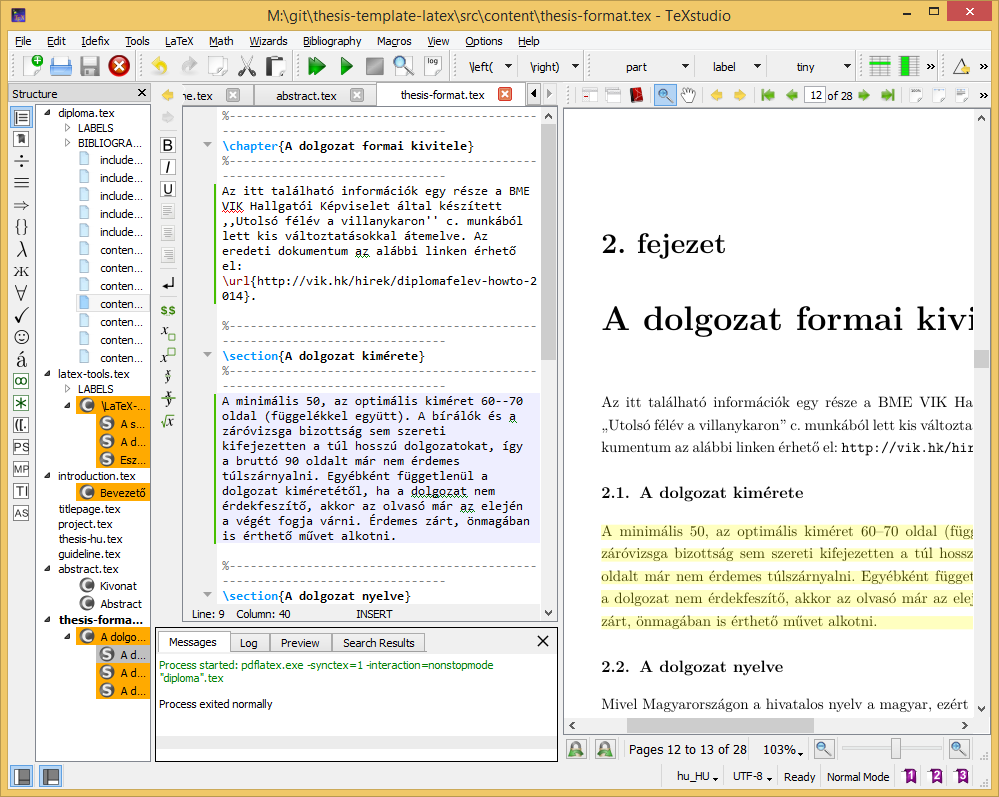
\includegraphics[width=150mm, keepaspectratio]{figures/TeXstudio.png}
\caption{A TeXstudio \LaTeX-szerkesztő.}
\label{fig:TeXstudio}
\end{figure}

A Property Sequence Chart[1] az MSC egy kiterjesztése. Sok új elemet vezet be ami nincs az MSC-ben, melyek megtekinthetők az 1. táblázaton, mint az üzenet típusokat: sima üzenet (e), elvárt üzenet (r) és nem kívánt üzenet (f). Így specifikálhatjuk, hogy mely üzenetek azok amik helyes viselkedésre utalnak és azok amelyek nem. Az elvárt üzenetek azok az üzenetek amelyeknek feltétetlen meg kell történiük a rendszer működése során. Egy sima üzenetnek nem jelent hibát a monitor szempontjából ha nem történik meg, viszont ha megjelenik, akkor a scenario-ban utána következő üzenetek ellenőrzésére kell áttérni. Szigorú sorrendezésre is ad megoldást a PSC, ami azt jelenti, hogy megadhatjuk explicit az üzenetek sorrendjét a követelményünkben. A PSC-ben egy üzenetre megkötést is rakhatunk. Megadhatjuk, hogy melyek azok az üzenetek amik nem kívántak az üzenetünk előtt vagy után. A különböző PSC tulajdonságok megtalálhatok a 2. ábrán.

\begin{figure}[!ht]
    \centering
    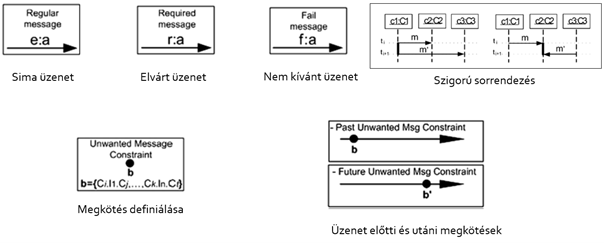
\includegraphics[width=150mm, keepaspectratio]{figures/2abra.png}
    \caption{A PSC különböző elemei[1].}
\end{figure}

Az üzeneteket a következő formában adjuk meg: Feladó.Üzenet.Címzett.

\begin{figure}[!ht]
    \centering
    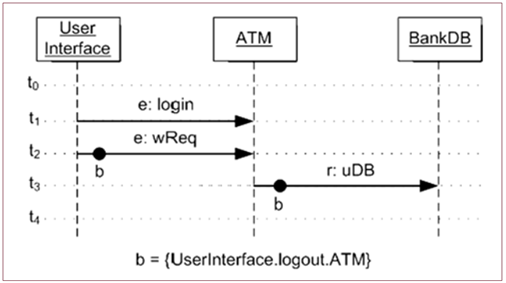
\includegraphics[width=150mm, keepaspectratio]{figures/3abra.png}
    \caption{PSC diagram egy ATM rendszer működésének az ellenőrzésére[1].}
\end{figure}
A 3. ábrán láthatunk egy példát arra, hogy egy követelményt hogyan lehet definiálni. Ez a PSC diagram egy ATM rendszer működését figyeli. Először a felhasználó egy login üzenettel bejelentkezik az ATM-be majd egy wReq üzenettel egy lekérdezést hajt végre. Ezen az üzeneten van egy megkötés, még pedig hogy az üzenet előtt nem történt kijelentkezés, logout. Az ATM ezután, ha nem történt logout egy elvárt üzenetet küld a Bank adatbázisába.

A scenario-ink specifikálására most már rendelkezésünkre áll egy grafikus nyelv. A következőkben az lesz a feladatunk, hogy ezeket a diagramokat úgy transzformáljunk, hogy monitor kódot lehessen belőlük készíteni.
